\chapter{Referencial Teórico}
\label{chap:modelo}

\section{Sistemas Distribuídos Ponto a Ponto}

As redes \textit{peer-to-peer}(também denominado \textit{p2p} ou ponto a ponto) são compostos de nós - computadores individuais - e, diferente dos sistemas de arquitetura centralizada, têm seus recursos computacionais (armazenamento, dados ou banda) compartilhados diretamente com todos os outros integrantes da rede, sem que haja um membro central que coordena todo o funcionamento. Portanto, permite que todos os nós detenham o mesmo poder, direitos e funções, sendo, simultaneamente, tanto fornecedores quanto consumidores de recursos \cite{Drescher2018}.

Esse tipo de arquitetura é propícia para o desenvolvimento de aplicações de compartilhamento de arquivos, distribuição de conteúdos e proteção de privacidade. A principal característica dos sistemas \textit{p2p} é a descentralização.

\begin{figure}[h]
	\centering
	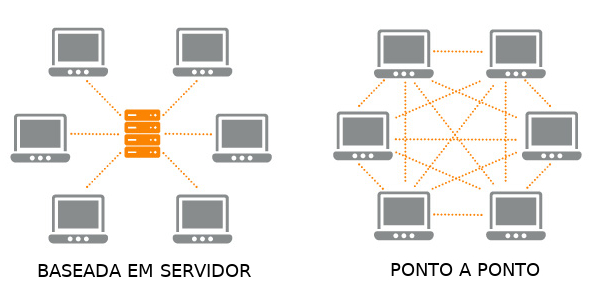
\includegraphics[width=\textwidth]{imagens/Server-based-vs-P2P-network.jpg}
	\caption{Rede com a arquitetura centralizada à esquerda e rede ponto a ponto à direita}
	Fonte: \cite{Wowza}
	\label{fig:redes}
\end{figure}

Na arquitetura centralizada, toda a rede fica dependente de um nó central, que fornecerá todos os recursos necessários para o funcionamento da rede. Esse nó detém todo o poder e controle, caso haja algum problema com ele, a rede ficará comprometida por completo. Já nas redes \textit{peer-to-peer}, isso não é um empecilho. Caso algum nó sofra com algum problema ou se desconecte voluntariamente da rede ou perca todas as informações, ninguém será afetado, todos continuarão realizando suas ações normalmente.

Apesar das vantagens, os sistemas ponto a ponto apresentam contrapartidas. Entre elas estão, principalmente, a integridade e confiança. Problemas estes que podem estar relacionados com falhas técnicas, nós mal intenciondos (usuários maliciosos), vulnerabilidade, integridade de informação, entre outros.
\section{Bitcoin}

O \textit{Bitcoin} geralmente é tratado como se fosse apenas uma moeda. Porém, o \textit{Bitcoin} é uma coleção de conceitos e tecnologias responsáveis por formar a base de todo um ecossistema um dinheiro digital. \cite{Antonopoulos2014} Dentro dessa variedade de conceitos que podem ser atribuídos a ele, podemos destacar três: (1) Um ativo digital (criptomoeda), (2) uma referência à tecnologia \textit{Blockchain} (livro-razão descentralizado) e (3) o protocolo que é executado sobre a tecnologia \textit{Blockchain} para descrever como os ativos são transferidos (\textit{softwares} que conduzem a transação) \cite{Swan2015}.

Todo esse sistema de pagamento de dinheiro digital foi lançado em 2009, sendo desenvolvido com um \textit{design} descentralizado e protegido por uma poderosa criptografia, tornando-o resiliente contra manipulações. \cite{Caetano2015} Os usuários possuem chaves que permitem com que eles provem a sua posse das moedas no decorrer das transações. Tais chaves são sempre armazenadas em uma carteira digital, a qual pode existir no computador do usuário, em sites de transações, em \textit{exchanges}, em \textit{hardwares}, ou em outras plataformas digitais. 

\section{Blockchain}

Assim, como o \textit{Bitcoin}, o \textit{Blockchain} também abrange um leque de significados, como: (1) uma terminologia para uma estrutura de dados, (2) o nome de um algoritmo, (3) um conjunto de tecnologias e (4) um termo abrangente para sistemas \textit{peer-to-peer} puramente distribuídos com uma área de aplicação comum.

Quando utilizado para nomear uma estrutura de dados, o termo refere-se a vários dados unidos em unidades chamadas de blocos. Tais blocos são conectados uns aos outros de forma encadeada, daí vem o nome \textit{Blockchain} (cadeia de blocos, em tradução livre). Quando atribuído a um algoritmo, o significado refere-se a um conjunto de instruções que lidam com o conteúdo de muitas estrutura de dados \textit{Blockchain} em um sistema \textit{p2p}. Ao se referir a um conjunto de tecnologias, o termo inclui a estrutura de dados, o algoritmo, tecnologias de criptografia e segurança os quais podem ser utilizados para prover integridade em sistemas puramente distribuídos ponto a ponto. E, diferente do significado anterior, a quarta atribuição ao termo é referente à um sistema distribuído como um todo, não unicamente a uma unidade de \textit{software} que faz parte desse tipo de sistema. \cite{Drescher2018}

O desenvolvimento desta tecnologia foi um avanço fundamental na ciência da computação, juntando cerca de quarenta anos de pesquisas em criptografia com vinte anos de pesquisas em moedas criptográficas. \cite{Swan2015} O Blockchain resolve um problema de longa data chamado “gasto duplo”. Este problema ocorre quando duas transações são aceitas com um montante que excede o valor antes disponível para gasto, ou seja, aquela quantia foi usada mais de uma vez.

Até o desenvolvimento do \textit{Blockchain}, o dinheiro digital não era escasso (assim como todos os outros recursos digitais), podendo ser copiados e replicados \textit{ad infinitum}, e não havia uma ­maneira de confirmar se aquele recurso já havia sido gasto sem que houvesse uma terceira parte envolvida para intermediar e realizar a sincronização entre todas as transações \cite{Swan2015}.

Para resolver o gasto duplo, o \textit{Blockchain} provê um mecanismo de confirmação e um livro-razão universal distribuído para que todos os nós (pontos) estejam informados e atualizados ao longo de cada transação. Cada informação nova adicionada na cadeia de blocos é armazenada em ordem cronológica, assim, fazendo com que o rastreamento seja feito de maneira simples. A cada 10 minutos um novo grupo de transações – ou seja, um bloco – é adicionado ao livro e todos os nós possuirão uma cópia do mesmo. Caso alguém tente usar o mesmo recurso mais de uma vez, será impossível, pois uma vez que a primeira operação dela foi iniciada, a mesma vai para um \textit{pool} de transações não confirmadas. Apenas a primeira das duas transações será confirmada e verificada pelos mineradores, enquanto a segunda será classificada como inválida e não terá confirmações suficientes para ser validada; e mesmo que as duas transações sejam feitas ao mesmo tempo, a que tiver mais confirmações dos mineradores (no mínimo seis, para que seis outros blocos sejam adicionados no topo do bloco que está sendo verificado) será a aceita.

A imagem abaixo mostra os passos para a realização de uma transação com \textit{Blockchain}. Primeiro, o usuário requisita uma transação. Em seguida, essa mesma requisição é transmitida para a rede, que será responsável por validar ou rejeitar o pedido de transação. Após isso, caso seja validada, ela é adicionada ao atual bloco de transações, o qual será encadeado com os outros blocos mais antigos, assim, confirmando a transação.

\begin{figure}[h]
	\centering
	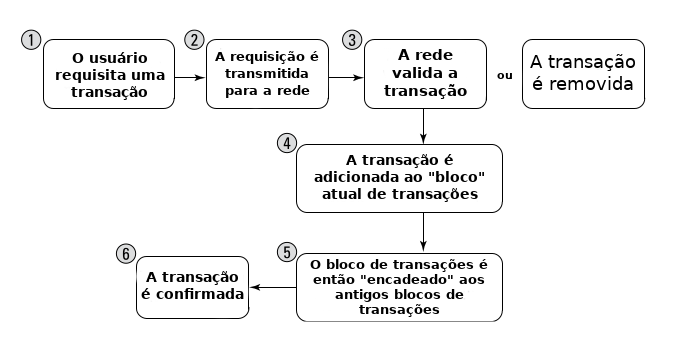
\includegraphics[width=\textwidth]{imagens/funcionamento-blockchain.png}
	\caption{Funcionamento do Blockchain}
	Fonte: \cite{Laurence2017}
	\label{fig:funcionamento-blockchain}
\end{figure}

A relação entre os sistemas \textit{p2p} e o \textit{Blockchain} é que o último serve para prover manter a integridade do primeiro sem que haja intermediação \cite{Drescher2018}.

\section{Exchanges}

As exchanges de criptoativos são plataformas digitais, com funcionamento
em tempo real que servem como intermediárias na compra, venda e troca dos mesmos, a fim de
facilitar o processo de aquisição. Elas costumam cobrar taxas nessas transações e organizar as 
informações de cada negociação em livros abertos. As exchanges são intermediários optativos, já
que, as criptomoedas podem funcionar de forma independente sem a necessidade de um intermediário envolvido no processo.

As seis \textit{exchanges} abordadas neste trabalho foram escolhidas com base no seu volume de transação e no nível de maturidade de sua \textit{API}. O volume é definido pela soma de todos os pares de mercado (\textit{market pairs}\footnote{\em Um \textit{market pair} é a cotação de duas moedas diferentes, com o valor de uma sendo cotado contra o valor de outra. O par é composto por uma moeda base e outra moeda de cotação.}) reportado pela corretora nas últimas vinte e quatro horas.

As informações a respeito do volume das corretoras são encontradas no \textit{Coin Market Cap}\footnote{\em https://coinmarketcap.com/rankings/exchanges/}, um \textit{site} que disponibiliza dados e gráficos em tempo real tanto das \textit{exchanges} quanto das criptomoedas existentes no mercado. No momento da escolha, as corretoras aqui analisadas estavam presentes entre as vinte primeiras posições no \textit{Coin Market Cap}.


\section{HTTP}

Projetado no início da década de 1990, o \textit{Hypertext Transfer Protocol} (Protocolo de Transferência de Hipertexto) é um protocolo de comunicação utilizado na transferência de documentos na \textit{Internet}. Ele garante a integridade dos dados transmitidos durante a comunicação. É por meio dele que as informações oriundas de servidores \textit{web} chegam de forma rápida, conveniente e confiável aos internautas, nos seus respectivos navegadores. O \textit{HTTP} segue o modelo de comunicação cliente-servidor, o qual o cliente inicia uma conexão com o servidor, realiza requisições e aguarda até receber alguma resposta.

\begin{figure}[h]
	\centering
	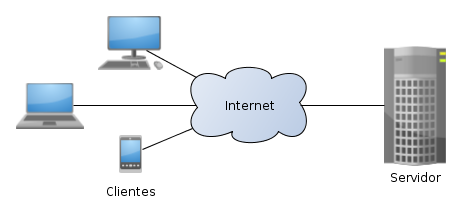
\includegraphics[width=\textwidth]{imagens/modelo-arquitetura-cliente-servidor.png}
	\caption{Modelo de arquitetura cliente-servidor}
	\cite{ClienteServidorWikipedia}
	\label{fig:modelo-arquitetura-cliente-servidor}
\end{figure}

\begin{figure}[h]
	\centering
	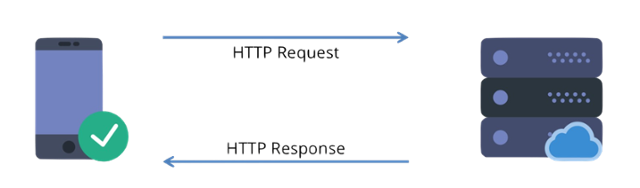
\includegraphics[width=\textwidth]{imagens/requisicao-http.png}
	\caption{Funcionamento de uma requisição HTTP}
	Fonte: \cite{HttpRequest}
	\label{fig:requisicao-http}
\end{figure}

Os servidores \textit{web} – também conhecidos como servidores \textit{HTTP} – são responsáveis por armazenar e prover todos os tipos de recursos \textit{web}: arquivos de texto, arquivos \textit{HTML}, arquivos de multimídia, etc.. O \textit{client} requisita ao \textit{server} o conteúdo desejado por meio de \textit{HTTP requests}  (requisições), e os servidores retornam os dados por meio de \textit{HTTP responses} (respostas) \cite{Gourley&Totty2002}, como mostrado na figura \ref{fig:requisicao-http}.

Além das características citadas, anteriormente, este protocolo é \textit{stateless}, ou seja, cada requisição é independente, mesmo que venham a ocorrer de forma simultânea e na mesma conexão cliente-servidor. Para o \textit{server}, cada \textit{request} é diferente, ele não guarda o estado das requisições anteriores, toda a informação é perdida.

\subsection{REST}

\textit{REST} é um acrônimo para \textit{Representational State Transfer} (Transferência de Estado Transacional), um estilo arquitetural para sistemas \textit{web} distribuídos a fim de facilitar a comunicação entre eles. Foi apresentado em 2000 por Roy Fielding, um dos autores da especificação do \textit{HTTP}, em sua tese de doutorado\footnote{\em https://www.ics.uci.edu/~fielding/pubs/dissertation/top.htm}. Nela, Roy sugeriu um conjunto de princípios, regras e \textit{constraints} que permitem o desenvolvimento de aplicações com interface bem definidas.
	
As aplicações desenvolvidas que seguem essa arquitetura são denominadas \textit{RESTful}, e seis princípios devem ser respeitados na implementação das mesmas:

\begin{itemize}
	\item \textbf{Cliente-servidor}: a portabilidade da interface do usuário e a escalabilidade do sistema  são melhoradas quando há uma separação do cliente, responsável pela interface, do servidor, que armazena as informações;
	\item \textbf{Stateless}: informações de sessão do usuário fica a cargo do cliente. Cada requisição para o servidor deve conter todas as informações necessárias para que ele entenda o \textit{request};
	\item \textbf{Armazenamento em cache}: requer que os dados em uma resposta sejam rotulados implícita ou explicitamente se podem ou não serem armazenados em \textit{cache}. Caso positivo, o cache do cliente poderá utilizar essas informações retornadas do servidor em outras requisições futuras;
	\item \textbf{Interface uniforme}: a fim de simplificar a arquitetura de todo o sistema, o \textit{REST} busca obter uma interface uniforme definindo quatro \textit{constraints}: identificação dos recursos, manipulação dos recursos através de representações, mensagens auto descritivas e hipermídia como motor do estado da aplicação;
	\item \textbf{Sistemas em camadas}: este modelo, também conhecido como \textit{layered systems}, permite que uma arquitetura seja composta de camadas hierárquicas, restringe o comportamento dos componentes de forma que cada um deles não possa acessar outras camadas além da qual eles estão interagindo no momento;
	\item \textbf{Código sob demanda}: este último princípio é optativo. Geralmente o usuário enviará as representações estáticas de recursos (\textit{JSON} ou \textit{XML}), porém, caso seja necessário, é possível retornar o código fonte executável para suportar parte da aplicação que está sendo desenvolvida.
\end{itemize}

\section{API}

\textit{Application Programming Interface} – Interface de Programação de Aplicações, em tradução livre – é um conjunto de definições, protocolos e ferramentas para o desenvolvimento e integração de \textit{softwares} de aplicações. Essa interface permite que o sistema possa se comunicar com produtos e serviços oferecidos por outras aplicações, dessa forma, simplificando e tornando mais flexível o processo de construção do sistema, consequentemente, gerando economia de tempo e de recursos.

Com as \textit{APIs}, a aplicação deixa disponível recursos, serviços e informações sem que haja uma perda na segurança e no controle, já que o acesso e as permissões serão especificadas pela equipe de desenvolvimento. Nos últimos anos, o \textit{REST} vem sendo o principal protocolo de padronização de \textit{APIs}.

\subsection{\textit{REST API: Design Rulebook}}

É o principal material utilizado neste trabalho como base para realizar as análises das \textit{APIs}. Segundo \cite{Masse:2016}, as regras servem para ajudar os desenvolvedores a construir \textit{RESTful APIs} consistentes que podem ser desfrutadas pelos usuários. Algumas delas tornaram-se padrões, de fato, outras era implícitas no protocolo \textit{HTTP}. Tais regras podem ser utilizadas por completo ou de forma separada, dependendo do contexto do serviço, e elas servem para responder algumas questões como:

\begin{itemize}
	\item Quando os caminhos da \textit{URI} devem ser nomeados com substantivos no plural?
	\item Quais métodos de requisição devem ser utilizados para atualizar o estado dos recursos?
	\item Como implementar operações diferentes do \textit{CRUD} nas \textit{URIs}?
	\item Qual é o código de \textit{status} \textit{HTTP} apropriado para um determinado cenário?
	\item Como gerenciar diferentes versões de uma representação do estado de um recurso?
	\item Como estruturar um \textit{hyperlink} em \textit{JSON}? 
\end{itemize}

\section{Trabalhos relacionados}

\subsection{\textit{API Management: An Architect’s Guide to Developing and Managing APIs for Your Organization}}

Este livro é um guia de como desenvolver, gerenciar e manter \textit{APIs} em sistemas corporativos. O autor aborda questões de segurança, ciclo de vida, documentação, padrões de projeto, controle de versão, monetização, \textit{analytics} e estratégias para testes de performance e testes de carga.

Na seção de seção de \textit{design} da interface da \textit{API}, princípios básicos do \textit{REST}, os verbos, os \textit{status codes}, a estrutura, convenções e boas práticas dos identificadores de recursos \textit{URIs}, versionamento, e outros detalhes importantes e necessários no projeto de construção de uma \textit{API}.

Segundo \cite{De2017}, as \textit{APIs} devem ser desenvolvidas para que tenham um longo ciclo de vida. Qualquer mudança acarreta em riscos de funcionamento para o cliente que a consome. Frequentes mudanças geralmente deixam usuários comuns e desenvolvedores frustrados. Utilizar padrões robustos na construção de \textit{APIs} ajuda a comunidade de desenvolvedores e pode salvar a companhia de ter despesas financeiras.

\subsection{\textit{REST API Development with Node.js: Manage and Understand the Full Capabilities of Successful REST Development}}

Assim como o trabalho anterior, neste livro o \cite{Doglio:2018} mostra todos os passos necessários para se desenvolver uma \textit{API} e lançá-la em um ambiente de produção. Nele, é feita uma introdução ao \textit{REST} e como desenvolver uma \textit{RESTful API} na linguagem \textit{Javascript} utilizando o \textit{framework Node.js}. A diferença encontra-se na abordagem das boas práticas de desenvolvimento de \textit{APIs}. O livro traz o conteúdo de forma mais superficial, não se aprofundando ou expondo os padrões minuciosamente. Por outro lado, o autor abordar o conteúdo didaticamente.

\subsection{\textit{API Design for C++}}

Este livro trata de forma mais profunda a construção de \textit{APIs} elegantes e robustas. Criar interfaces de alta qualidade é, portanto, uma habilidade essencial de engenharia e o foco central deste trabalho. \cite{Reddy2011}

Para auxiliar na performance, o autor utiliza a linguagem de programação \textit{C++}, que permite que a aplicação seja processada até mesmo em unidades de processamento gráfico (GPU). Alguns componentes para aumentar o desempenho das \textit{APIs} são considerados, entre eles: velocidade do tempo de compilação, velocidade do tempo de execução, sobrecarga da memória em tempo de execução, tamanho da aplicação e o tempo de inicialização.

Além do desempenho da aplicação, o livro aborda os diferentes tipos de \textit{patterns} de implementação e possui uma seção que trata da qualidade de uma \textit{API}, descrevendo as caracteríticas que uma boa aplicação deve ter, entre elas: modelagem do domínio do problema, esconder os detalhes de implementação, ser fácil de utilização, ser testada, documentada e estável.
